\section{Hypothèse de pertinence}
\label{section:4.4-HYPOTHESE-PERTINENCE}

	%%% Introduction / Transition.
	Jusqu'à présent, nous avons analysé la performance et l'évolution des résultats de notre implémentation du \textit{clustering} interactif à l'aide d'une vérité terrain (cf. calcul de \texttt{v-measure}).
	Cependant, une telle référence n'est pas accessible en situation réelle (l'objectif de notre méthode est précisément de la construire).
	Nous devons donc nous intéresser à d'autres moyens d'estimer la pertinence des bases d'apprentissages obtenus et de définir comment définir l'exploitabilité d'un résultat.
	Ainsi, nous aimerions vérifier l'hypothèse suivante :
	
	%%% Formulation des hypothèses:
	\begin{tcolorbox}[
		title=\faVial~\textbf{Hypothèse de pertinence}~\faVial,
		colback=colorTcolorboxHypothesis!15,
		colframe=colorTcolorboxHypothesis!75,
		width=\linewidth
	]
		« \textbf{
			Au cours d'une méthodologie d'annotation basée sur le \textit{clustering} interactif, il est possible à un expert métier d'évaluer rapidement la pertinence de la base d'apprentissage en construction sans utiliser de vérité terrain.
		} » \\
		
		% Figure.
		La figure~\ref{figure:4.4-HYPOTHESE-PERTINENCE} illustre cette hypothèse et l'espoir de pouvoir caractériser la qualité de la base d'apprentissage en cours de construction en fonction d'une valeur métier exprimée par un expert.
		%
		\begin{figure}[H]  % keep [H] to be in the tcolorbox.
			\centering
			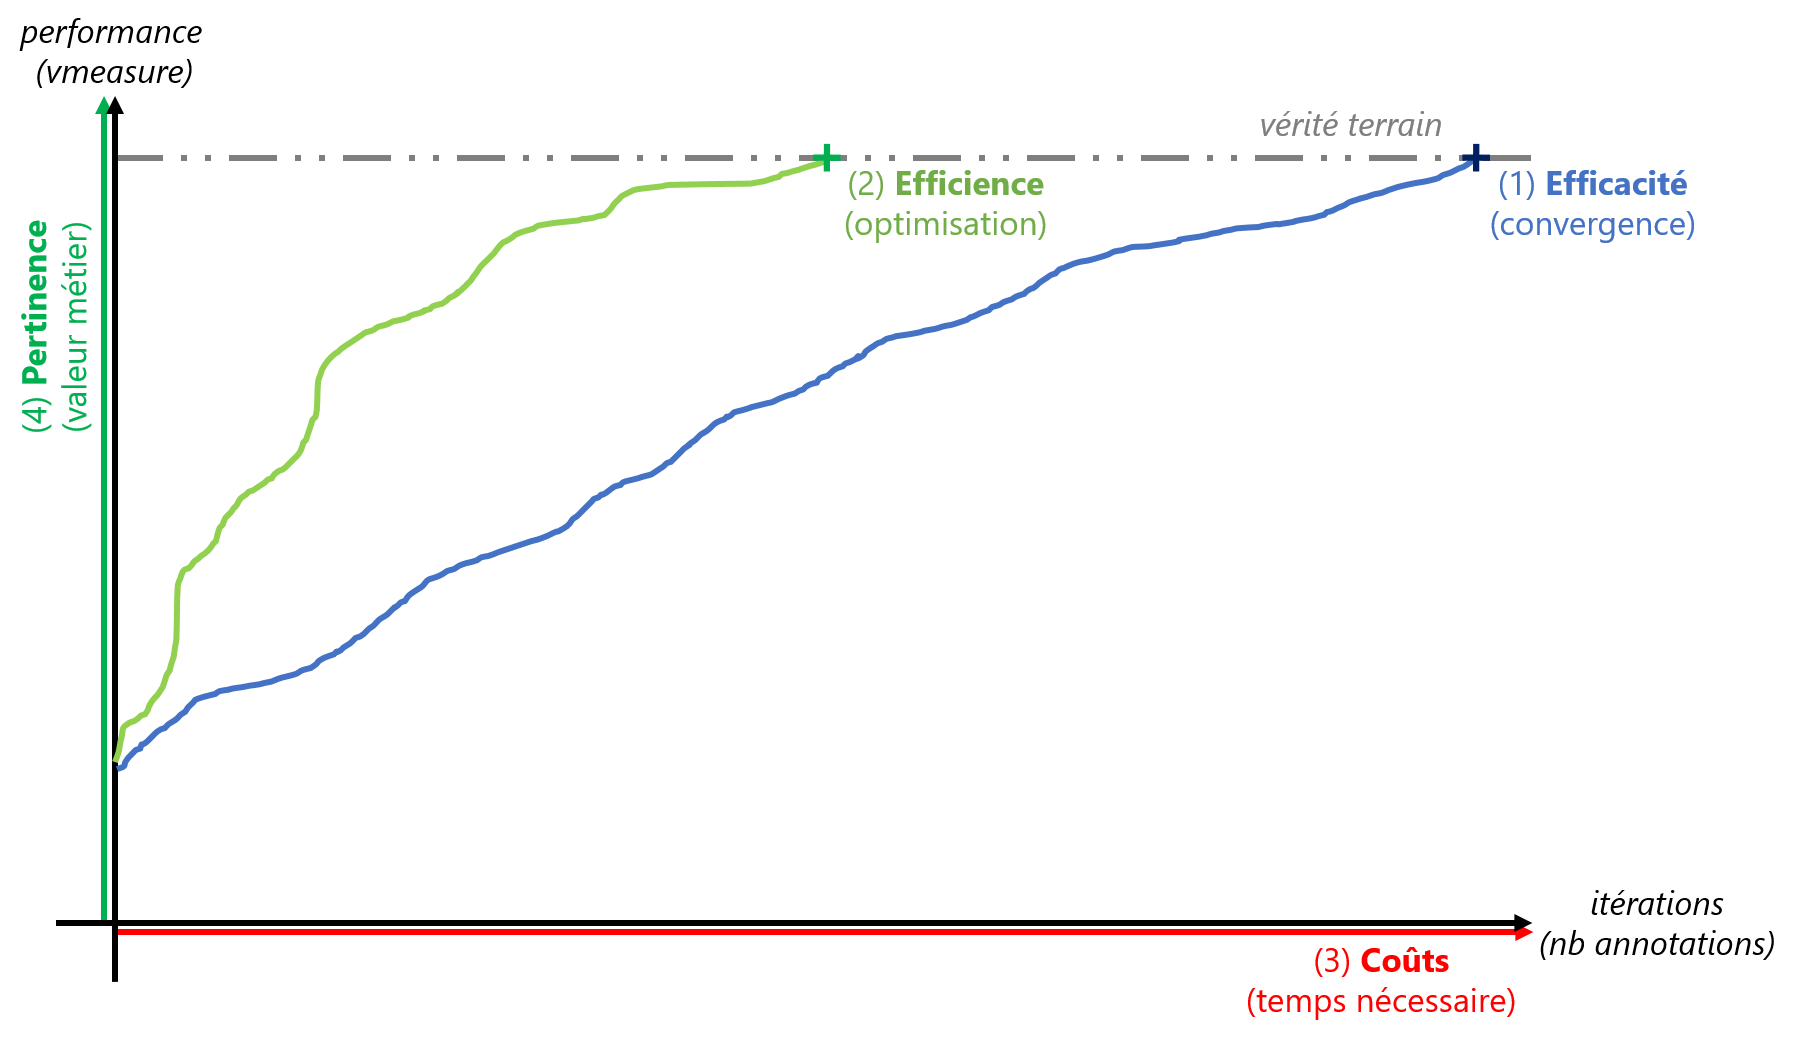
\includegraphics[width=0.95\textwidth]{figures/hypotheses-04-pertinence}
			\caption{Illustration des études réalisées sur le \textit{clustering} interactif (\textit{étape 4/6}) en schématisant l'évolution de la pertinence (\textit{valeur métier évaluée par l'expert et exprimé en nombre de clusters}) d'une base d'apprentissage en cours de construction en fonction du coût temporel de la méthode (\textit{temps nécessaire à l'expert métier et à la machine}).}
			\label{figure:4.4-HYPOTHESE-PERTINENCE}
		\end{figure}

	\end{tcolorbox}
		
	% Résumé de l'étude.
	Afin de vérifier cette hypothèse, nous explorons trois approches :
	\begin{itemize}
		\item une \textbf{vérification par un expert} du partitionnement des données obtenus, en parcourant manuellement le contenu des \textit{clusters} et en donnant un avis sur l'exploitabilité de ces derniers (cf. sous-section~\ref{section:4.4.1-ETUDE-PERTINENCE-VERIFICATION-MANUELLE}) ;
		\item une analyse des \textbf{patterns linguistiques saillants} dans la base d'apprentissage à l'aide d'une stratégie de sélection des composantes principales d'un modèle (cf. sous-section~\ref{section:4.4.2-ETUDE-PERTINENCE-PATTERNS-LINGUISTIQUES}),
		\item et une approche utilisant un \textbf{résumé automatique de thématique} par un modèle de langue, permettant de décrire succinctement le contenu des \textit{clusters} en une phrase. (cf. sous-section~\ref{section:4.4.3-ETUDE-PERTINENCE-RESUME-AUTOMATIQUE}).
	\end{itemize}
	
	
	%%%
	%%% Subsection 4.4.1: Étude d'une vérification manuelle de la valeur métier d'une base d'apprentissage par un expert
	%%%
	\subsection{Étude d'une vérification manuelle de la valeur métier d'une base d'apprentissage par un expert}
	\label{section:4.4.1-ETUDE-PERTINENCE-VERIFICATION-MANUELLE}
		
		% Objectif de l'expérience.
		\todo[inline]{A REDIGER: objectif de l'expérience}
		Afin d'estimer la pertinence d'un résultat de \textit{clustering}, notre première intuition consiste à demander l'avis d'un expert sur la base d'apprentissage en cours de construction.
	
		%%% Protocole expérimental.
		\subsubsection{Protocole expérimental}
			\todo[inline]{A REDIGER}
			% Axiome.
			% Pseudo-code.
			% Détails de l'expérience.
			% Référence scripts.

		%%% Résultats
		\subsubsection{Résultats obtenus}
			\todo[inline]{A REDIGER}
		
			% Description statistiques.
			\todo[inline]{A REDIGER: On peut voir 3 phases: INEXPLOITABLE / DE PLUS EN PLUS EXPLOITABLE / EXPLOITABLE ; les partiellement exploitables servent de transition.}
			
			% Exemple.
			\todo[inline]{A REDIGER: tableau avec exemples ?}
			
			% Figure.
			%
			\begin{figure}[!htb]
				\centering
				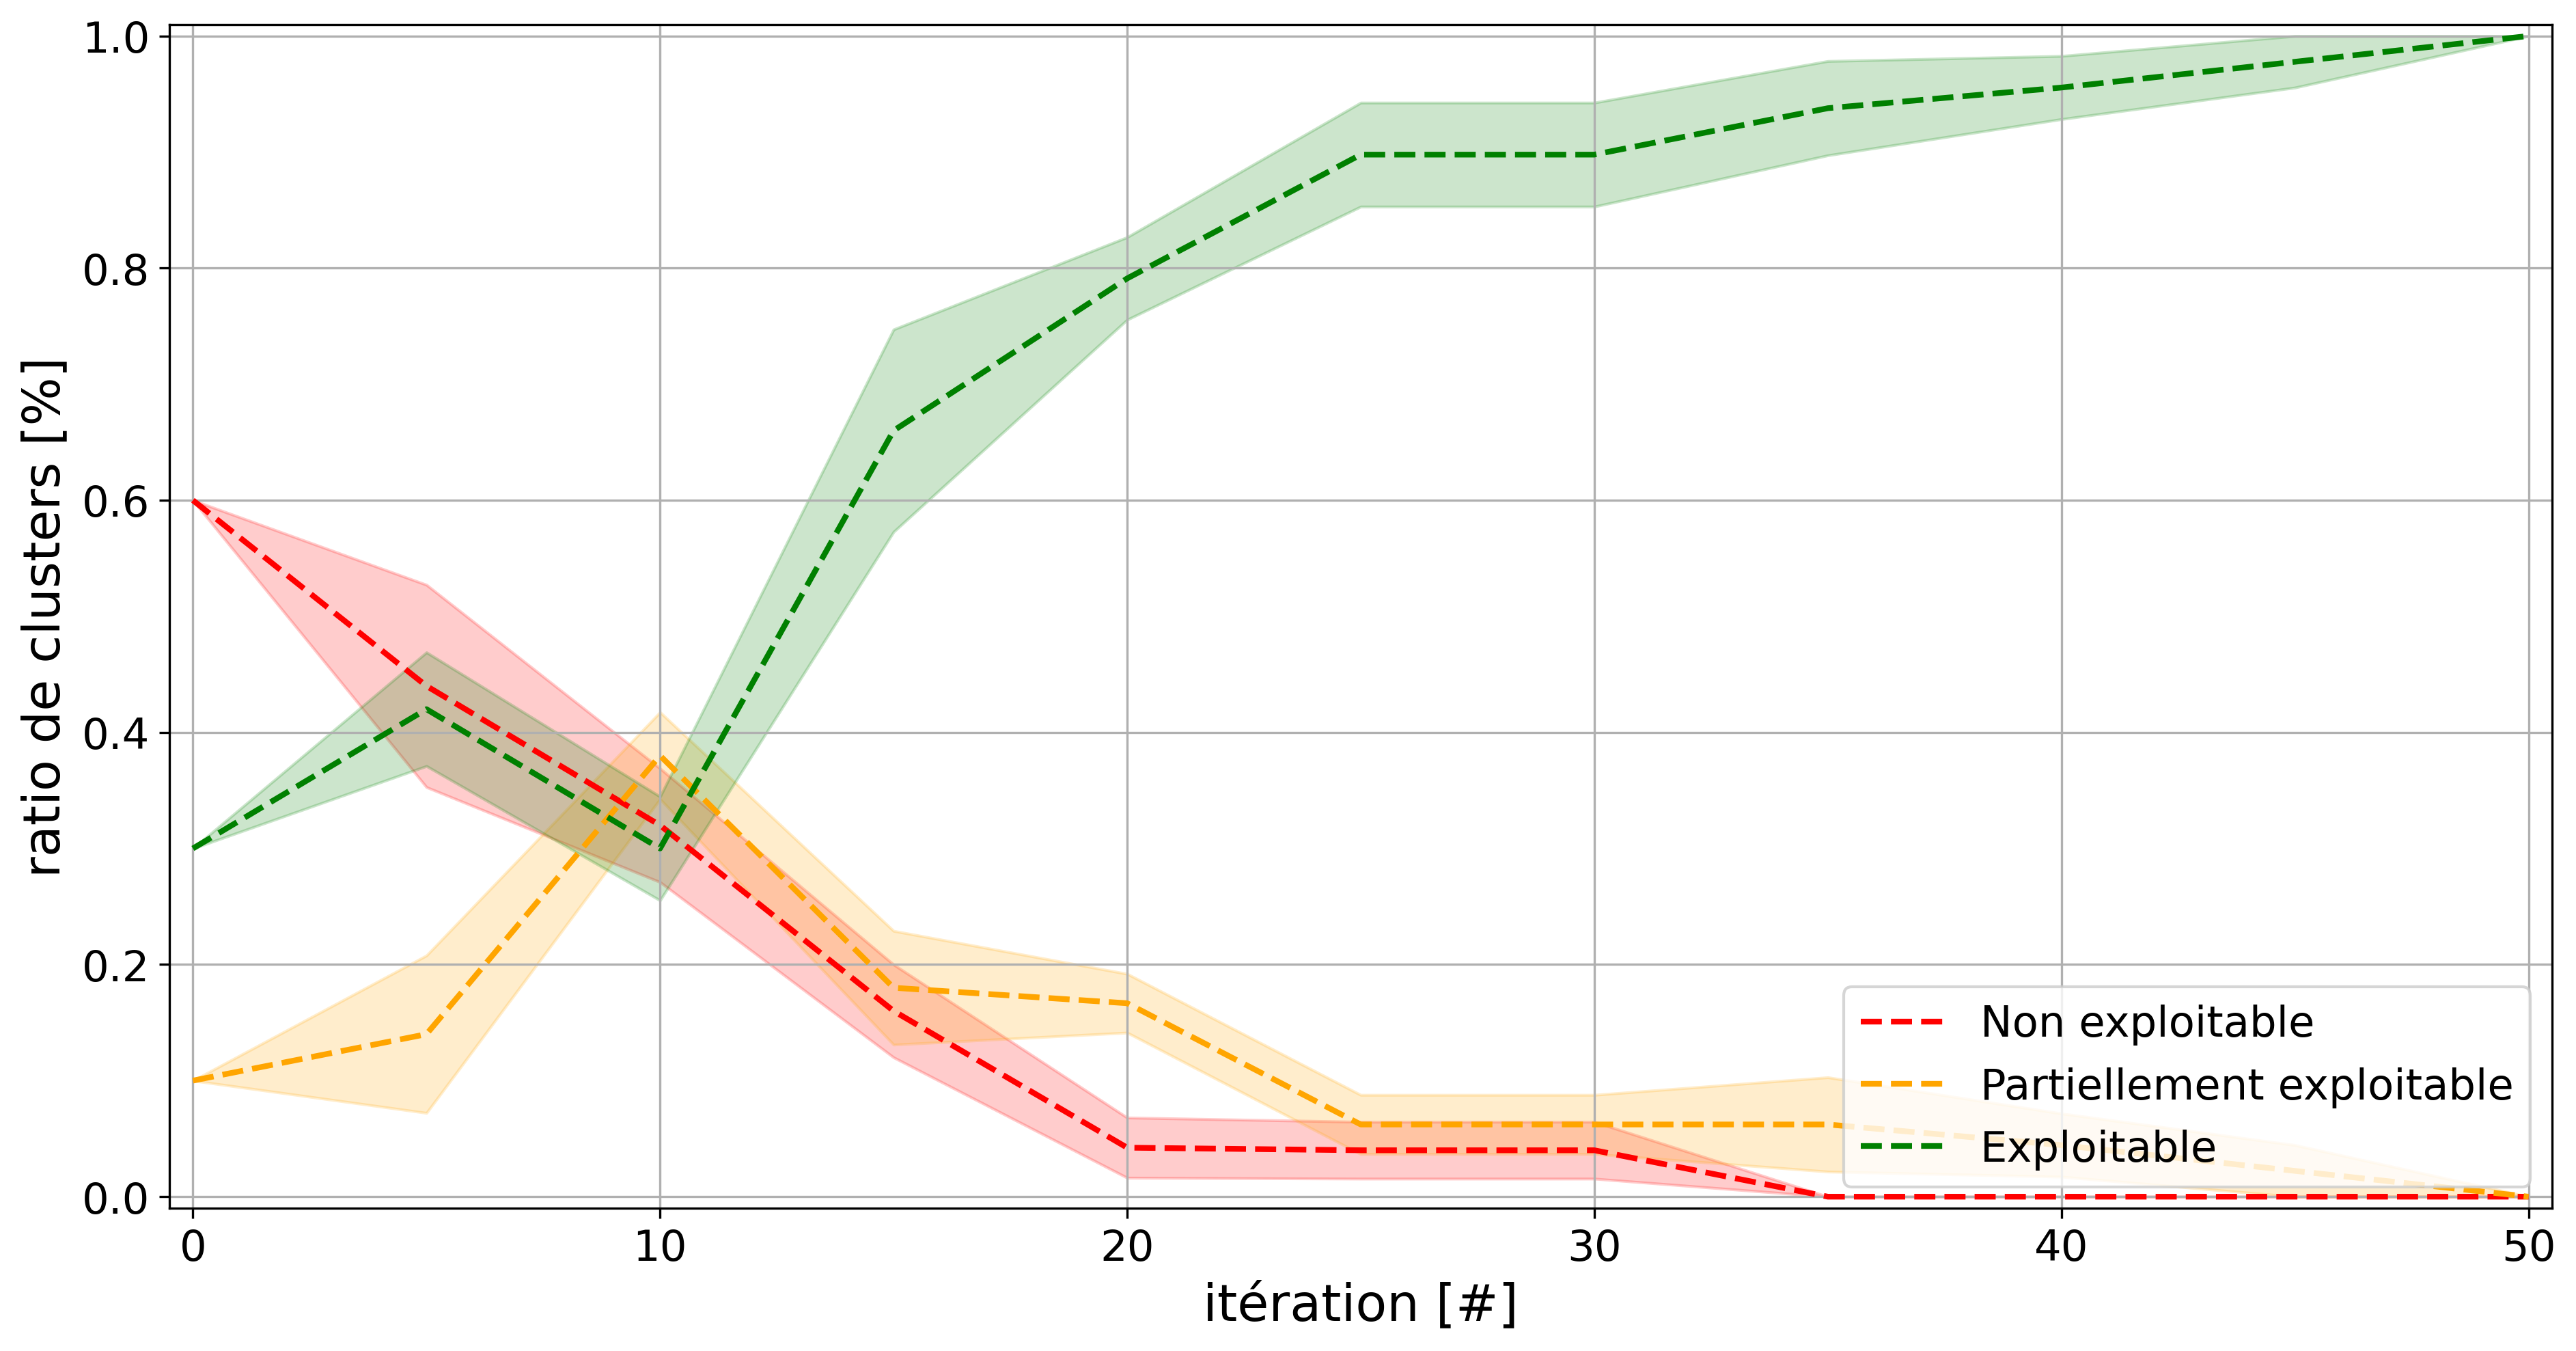
\includegraphics[width=0.95\textwidth]{figures/etude-pertinence-llm-check-clustering-annotation-favori}
				\caption{Évolution de la pertinence métier moyenne d'un résultat en fonction du nombre d'itérations de la méthode.
				La pertinence est estimée manuellement en trois niveaux (\texttt{non exploitable}, \texttt{partiellement exploitable} et \texttt{exploitable}) sur la base du contenu des \textit{clusters} et est exprimée en proportion du nombre de \textit{clusters} concernés.}
				\label{figure:4.4.1-ETUDE-PERTINENCE-VERIFICATION-MANUELLE}
			\end{figure}

		%%% Discussion
		\subsubsection{Discussion}
			\todo[inline]{A REDIGER}
		
			% Remaques expérience utilisateur.
			\todo[inline]{A REDIGER: C'est super fastidieux, sensible à l’inattention, ...}
			
			% Conclusions et suggestion.
	
	
	%%%
	%%% Subsection 4.4.2: Etude des patterns linguistiques pertinents à l'aide de la \textit{Features Maximization}
	%%%
	\subsection{Étude des patterns linguistiques pertinents à l'aide de la \textit{Features Maximization}}
	\label{section:4.4.2-ETUDE-PERTINENCE-PATTERNS-LINGUISTIQUES}
		
		% Objectif de l'expérience.
		\todo[inline]{A REDIGER: objectif de l'expérience}
	
		%%% Protocole expérimental.
		\subsubsection{Protocole expérimental}
			\todo[inline]{A REDIGER}
			% Axiome.
			% Pseudo-code.
			% Détails de l'expérience.
			% Référence scripts.

		%%% Résultats
		\subsubsection{Résultats obtenus}
			\todo[inline]{A REDIGER}
		
			% Description statistiques.
			
			% Exemple.
			\todo[inline]{A REDIGER: tableau avec exemples ?}

		%%% Discussion
		\subsubsection{Discussion}
			\todo[inline]{A REDIGER}
		
			% Remaques expérience utilisateur.
			\todo[inline]{A REDIGER: C'est pas adapté pour un expert métier, mais ça peut être utilisé pour de l'affichage}
			
			% Exemple.
			\todo[inline]{A REDIGER: tableau avec exemples ?}
			
			% Conclusions et suggestion.
	
	
	
	%%%
	%%% Subsection 4.4.3: Etude d'un résumé automatique des \textit{clusters} à l'aide d'un modèle de langue.
	%%%
	\subsection{Étude d'un résumé automatique des \textit{clusters} à l'aide d'un modèle de langue}
	\label{section:4.4.3-ETUDE-PERTINENCE-RESUME-AUTOMATIQUE}
		
		% Objectif de l'expérience.
		\todo[inline]{A REDIGER: objectif de l'expérience}
	
		%%% Protocole expérimental.
		\subsubsection{Protocole expérimental}
			\todo[inline]{A REDIGER}
			% Axiome.
			% Pseudo-code.
			% Détails de l'expérience.
			% Référence scripts.

		%%% Résultats
		\subsubsection{Résultats obtenus}
			\todo[inline]{A REDIGER}
		
			% Description statistiques.
			\todo[inline]{A REDIGER: On peut voir 3 phases: INEXPLOITABLE / DE PLUS EN PLUS EXPLOITABLE / EXPLOITABLE ; les partiellement exploitables sont pas très présents.}
			
			% Exemple.
			\todo[inline]{A REDIGER: tableau avec exemples ?}
			
			% Figure.
			%
			\begin{figure}[!htb]
				\centering
				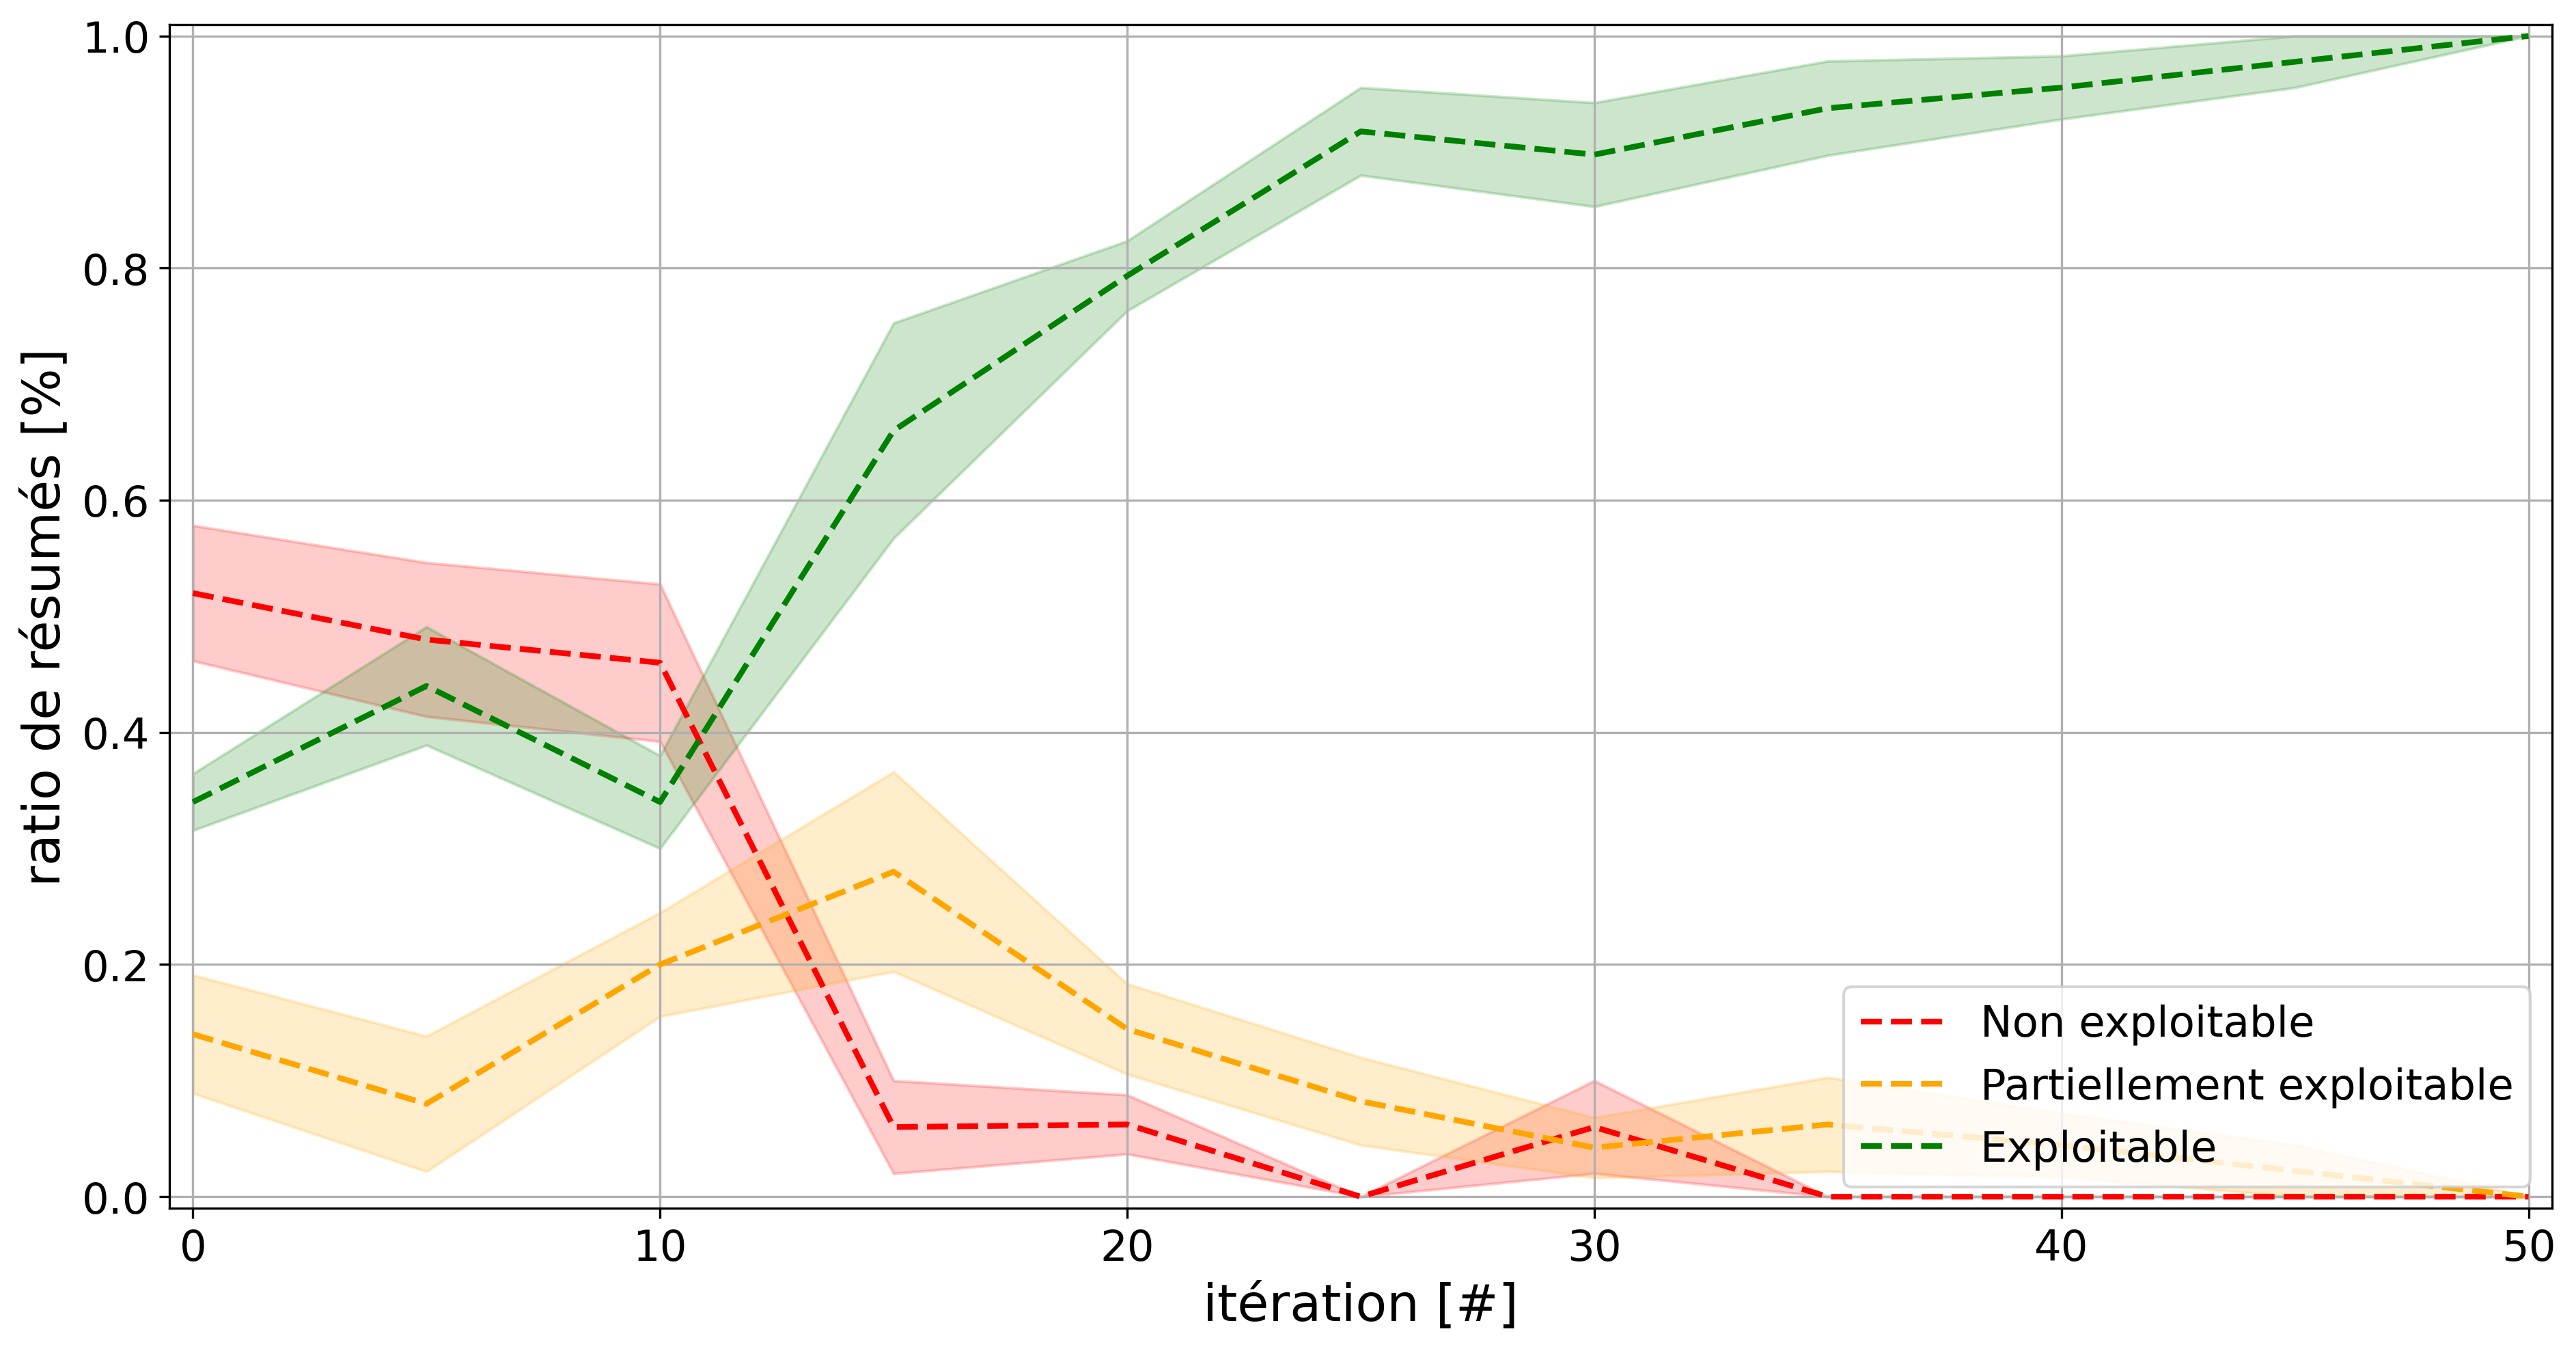
\includegraphics[width=0.95\textwidth]{figures/etude-pertinence-llm-check-resume-annotation-favori}
				\caption{Évolution de la pertinence métier moyenne d'un résultat en fonction du nombre d'itérations de la méthode.
				La pertinence est estimée en trois niveaux (\texttt{non exploitable}, \texttt{partiellement exploitable} et \texttt{exploitable}) sur la base du résumé automatique des \textit{clusters} par un modèle de langue et est exprimée en proportion du nombre de \textit{résumés} concernés.}
				\label{figure:4.4.3-ETUDE-PERTINENCE-RESUME-AUTOMATIQUE}
			\end{figure}

		%%% Discussion
		\subsubsection{Discussion}
			\todo[inline]{A REDIGER}
		
			% Remaques expérience utilisateur.
			\todo[inline]{A REDIGER: C'est super pratique, super accessible}
			\todo[inline]{A REDIGER: C'est parfois un peu ambigu...}
			
			% Conclusions et suggestion.
	
	
	%%%
	%%% Subsection 4.4.4: Étude de la cohérence statistique de la base d'apprentissage en cours de construction
	%%%
	%\subsection{Étude de la cohérence statistique de la base d'apprentissage en cours de construction}
	%\label{section:4.4.4-ETUDE-PERTINENCE-COHERENCE}
	%	
	%	% Objectif de l'expérience.
	%	\todo[inline]{A REDIGER: objectif de l'expérience}
	%
	%	%%% Protocole expérimental.
	%	\subsubsection{Protocole expérimental}
	%		\todo[inline]{A REDIGER}
	%		% Axiome.
	%		% Pseudo-code.
	%		% Détails de l'expérience.
	%		% Référence scripts.
	%
	%	%%% Résultats
	%	\subsubsection{Résultats obtenus}
	%		\todo[inline]{A REDIGER}
	%	
	%		% Description statistiques.
	%		
	%		% Exemple.
	%		
	%		% Figure.
	%		%
	%		\begin{figure}[!htb]
	%			\centering
	%			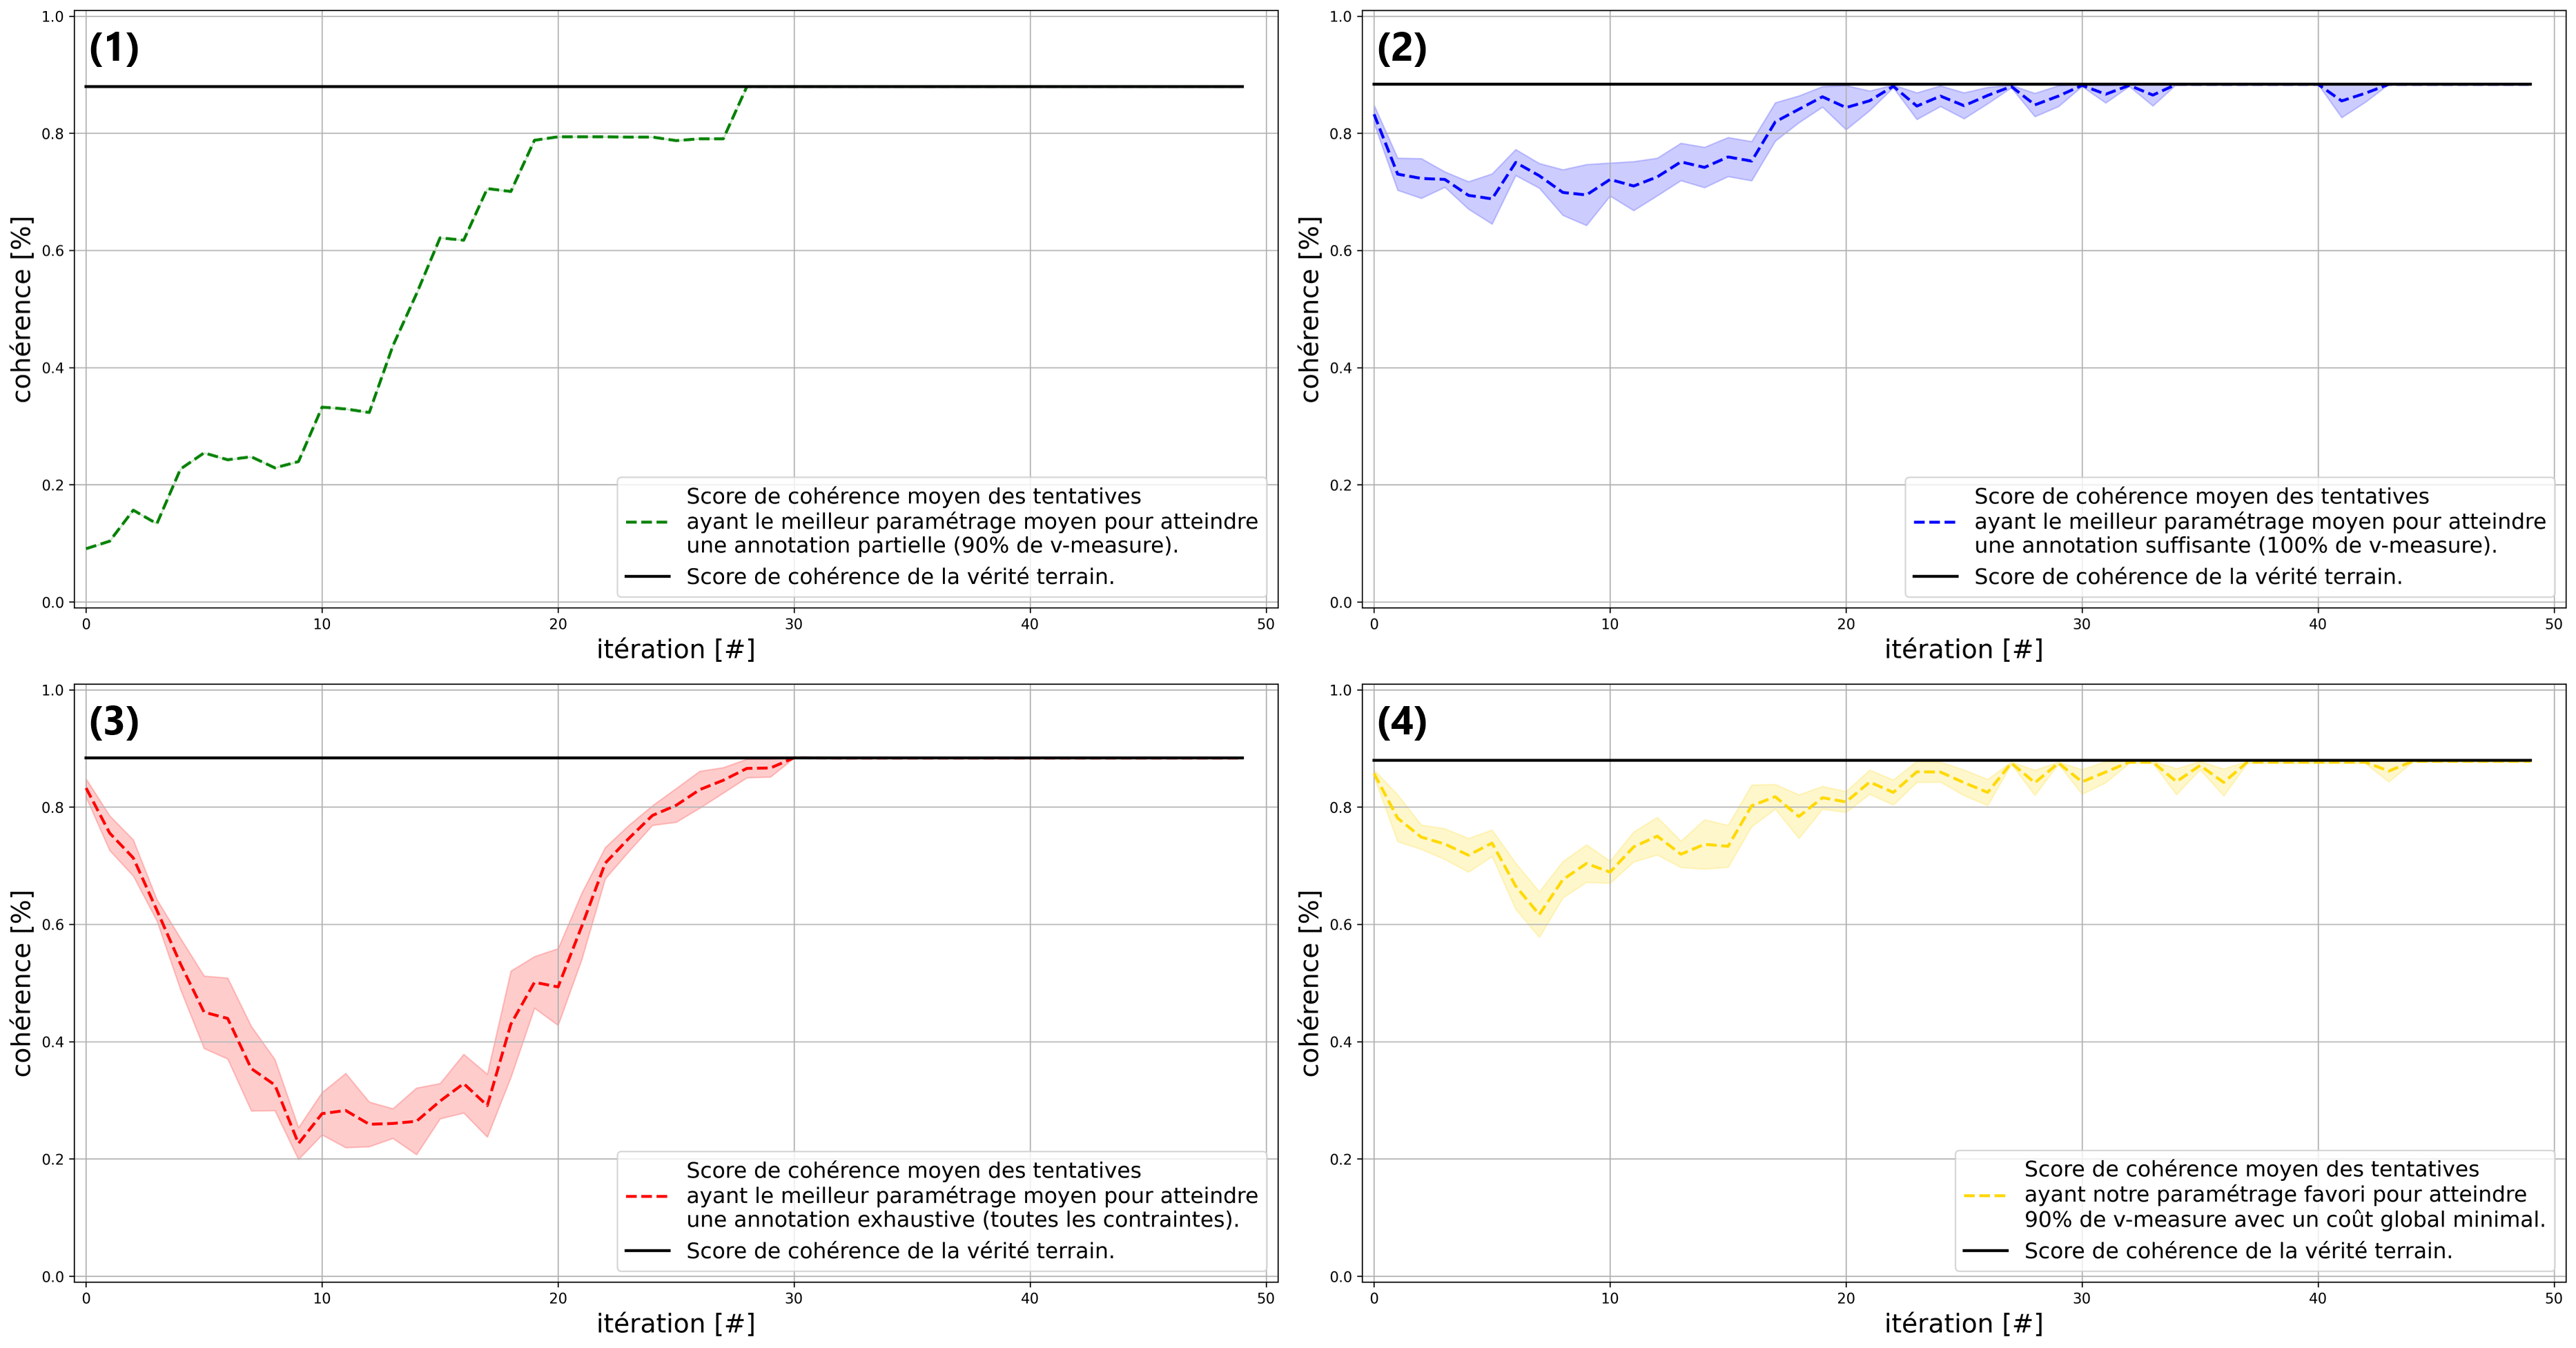
\includegraphics[width=0.95\textwidth]{figures/etude-pertinence-consistence}
	%			\caption{Évolution du score de cohérence moyen des tentatives en fonction de leur paramétrage : \textbf{(1)} meilleur paramétrage moyen une annotation partielle (\texttt{90}\% de \texttt{v-measure}), \textbf{(2)} meilleur paramétrage moyen une annotation suffisante (\texttt{100}\% de \texttt{v-measure}), \textbf{(3)} meilleur paramétrage moyen une annotation exhaustive (annoter toutes les contraintes possibles), et \textbf{(4)} paramétrage favori (\texttt{90}\% de \texttt{v-measure} avec un coût minimal). \\
	%			Note : \textit{Le score de cohérence de la vérité terrain peut varier en fonction des méthodes de prétraitements et de vectorisation utilisées.}}
	%			\label{figure:4.4.4-ETUDE-PERTINENCE-COHERENCE-ANNOTATION}
	%		\end{figure}
	%
	%	%%% Discussion
	%	\subsubsection{Discussion}
	%		\todo[inline]{A REDIGER}
	%	
	%		% Remaques expérience utilisateur.
	%		
	%		% Conclusions et suggestion.